\section{Iterator}

This iterator pattern is a pattern used to get access to the elements of a collection in a object secuentially without the need to know or expose its underlying representation.

% Description of the design pattern

\subsection*{Role}

The Iterator pattern here plays the role to secure the elements of the collections. SimplePrincipalCollection play the role of the internal design of the iterator, while the DelegatingSubject is the security layer that handles the collection and the other interfaces that extend the collections withouth exposing all elements of the collection.

\subsection*{Example}

\begin{center}
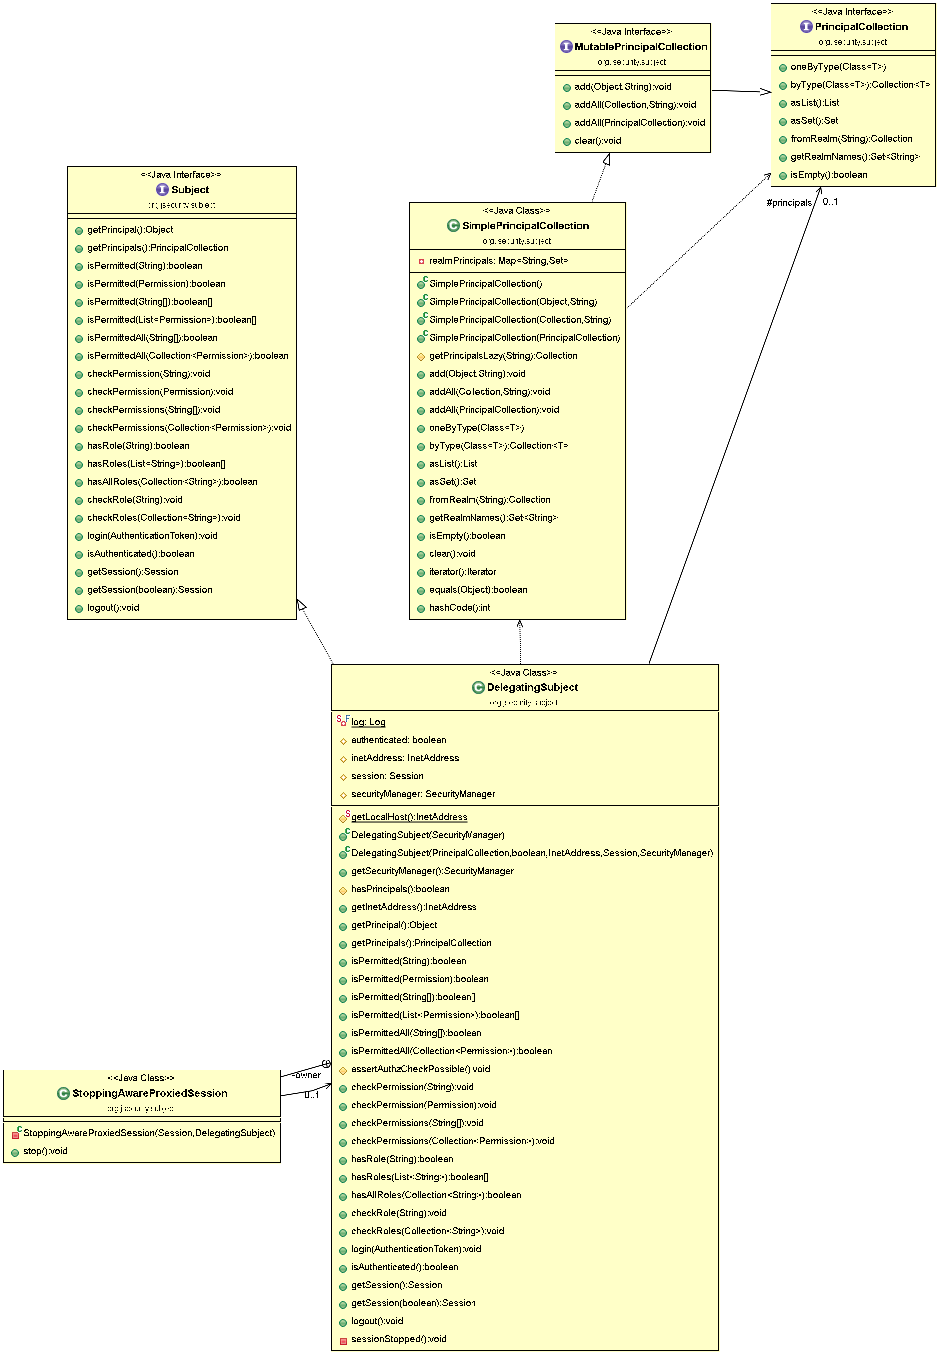
\includegraphics[width=16cm, height=19cm]{images/iterator.png}
\end{center}

In the program "18_jsecurity" in "org.jsecurity.subject/SimplePrincipalCollection" class that implements the MutablePrincipalCollection in which they implement an internal design of the iterator for the collection:

\begin{figure}[!tbp]
\centering
\lstset{language=Java, stepnumber=1, showspaces=false, showstringspaces=false,breaklines=true}
\begin{lstlisting}

public class SimplePrincipalCollection implements MutablePrincipalCollection {

    private Map<String, Set> realmPrincipals;

    public SimplePrincipalCollection() {
    }

    public SimplePrincipalCollection(Object principal, String realmName) {
        if (principal instanceof Collection) {
            addAll((Collection) principal, realmName);
        } else {
            add(principal, realmName);
        }
    }

    public SimplePrincipalCollection(Collection principals, String realmName) {
        addAll(principals, realmName);
    }

    public SimplePrincipalCollection(PrincipalCollection principals) {
        addAll(principals);
    }

    protected Collection getPrincipalsLazy(String realmName) {
        if (realmPrincipals == null) {
            realmPrincipals = new LinkedHashMap<String, Set>();
        }
        Set principals = realmPrincipals.get(realmName);
        if (principals == null) {
            principals = new LinkedHashSet();
            realmPrincipals.put(realmName, principals);
        }
        return principals;
    }

    public void add(Object principal, String realmName) {
        if (realmName == null) {
            throw new IllegalArgumentException("realmName argument cannot be null.");
        }
        if (principal == null) {
            throw new IllegalArgumentException("principal argument cannot be null.");
        }
        getPrincipalsLazy(realmName).add(principal);
    }

    public void addAll(Collection principals, String realmName) {
        if (realmName == null) {
            throw new IllegalArgumentException("realmName argument cannot be null.");
        }
        if (principals == null) {
            throw new IllegalArgumentException("principals argument cannot be null.");
        }
        if (principals.isEmpty()) {
            throw new IllegalArgumentException("principals argument cannot be an empty collection.");
        }
        getPrincipalsLazy(realmName).addAll(principals);
    }

    public void addAll(PrincipalCollection principals) {
        if (principals.getRealmNames() != null) {
            for (String realmName : principals.getRealmNames()) {
                for (Object principal : principals.fromRealm(realmName)) {
                    add(principal, realmName);
                }
            }
        }
    }

    public <T> T oneByType(Class<T> type) {
        if (realmPrincipals == null || realmPrincipals.isEmpty()) {
            return null;
        }
        Collection<Set> values = realmPrincipals.values();
        for (Set set : values) {
            for (Object o : set) {
                if (type.isAssignableFrom(o.getClass())) {
                    return (T) o;
                }
            }
        }
        return null;
    }

    public <T> Collection<T> byType(Class<T> type) {
        if (realmPrincipals == null || realmPrincipals.isEmpty()) {
            return Collections.EMPTY_SET;
        }
        Set<T> typed = new LinkedHashSet<T>();
        Collection<Set> values = realmPrincipals.values();
        for (Set set : values) {
            for (Object o : set) {
                if (type.isAssignableFrom(o.getClass())) {
                    typed.add((T) o);
                }
            }
        }
        if (typed.isEmpty()) {
            return Collections.EMPTY_SET;
        }
        return Collections.unmodifiableSet(typed);
    }

    public List asList() {
        Set all = asSet();
        if (all.isEmpty()) {
            return Collections.EMPTY_LIST;
        }
        return Collections.unmodifiableList(new ArrayList(all));
    }

    public Set asSet() {
        if (realmPrincipals == null || realmPrincipals.isEmpty()) {
            return Collections.EMPTY_SET;
        }
        Set aggregated = new LinkedHashSet();
        Collection<Set> values = realmPrincipals.values();


    public Iterator iterator() {
        return asSet().iterator();
    }
\end{lstlisting}
\caption{SimplePrincipalColletion.java}
\label{SimplePrincipalColletion}
\end{figure}

In the interface in MutablePrincipalCollection, we can see it extends the principal collection adding all the principals to the given collection.

\begin{figure}[!tbp]
\centering
\lstset{language=Java, stepnumber=1, showspaces=false, showstringspaces=false,breaklines=true}
\begin{lstlisting}

public interface MutablePrincipalCollection extends PrincipalCollection {

    void add(Object principal, String realmName);

     void addAll(Collection principals, String realmName);

    void addAll(PrincipalCollection principals);


    void clear();
}
\end{lstlisting}
\caption{AttributeModelBuilder.java}
\label{AttributeModelBuilder}
\end{figure}

In the interface PrincipalCollection they return the collection info necessary in different functions:

\begin{figure}[!tbp]
\centering
\lstset{language=Java, stepnumber=1, showspaces=false, showstringspaces=false,breaklines=true}
\begin{lstlisting}

public interface PrincipalCollection extends Iterable, Serializable {

    <T> T oneByType(Class<T> type);
    <T> Collection<T> byType(Class<T> type);
    List asList();
    Set asSet();
    Collection fromRealm(String realmName);
    Set<String> getRealmNames();
    boolean isEmpty();
}

\end{lstlisting}
\caption{PrincipalCollection.java}
\label{PrincipalCollection}
\end{figure}

The DelegatingSubject class, delegates the method calls and iterates the objects withouth exposing the whole colection:

\begin{figure}[!tbp]
\centering
\lstset{language=Java, stepnumber=1, showspaces=false, showstringspaces=false,breaklines=true}
\begin{lstlisting}

    public DelegatingSubject(PrincipalCollection principals, boolean authenticated, InetAddress inetAddress,
                             Session session, SecurityManager securityManager) {
        if (securityManager == null) {
            throw new IllegalArgumentException("SecurityManager argument cannot be null.");
        }
        this.securityManager = securityManager;
        this.principals = principals;

        this.authenticated = authenticated;

        if (inetAddress != null) {
            this.inetAddress = inetAddress;
        } else {
            this.inetAddress = getLocalHost();
        }
        if (session != null) {
            this.session = new StoppingAwareProxiedSession(session, this);
        }
    }
    public Object getPrincipal() {
        PrincipalCollection principals = getPrincipals();
        if (principals == null || principals.isEmpty()) {
            return null;
        }
        return principals.asSet().iterator().next();
    }

    public PrincipalCollection getPrincipals() {
        return this.principals;
    }

\end{lstlisting}
\caption{DelegatingSubject.java}
\label{DelegatingSubject}
\end{figure}

The Subject interface just gets the Objects and Principal Collection and check the role of each element:

\begin{figure}[!tbp]
\centering
\lstset{language=Java, stepnumber=1, showspaces=false, showstringspaces=false,breaklines=true}
\begin{lstlisting}
public interface Subject {

    Object getPrincipal();
    PrincipalCollection getPrincipals();
    boolean hasAllRoles(Collection<String> roleIdentifiers);
    void checkRole(String roleIdentifier) throws AuthorizationException;
    void checkRoles(Collection<String> roleIdentifiers) throws AuthorizationException;

...
}
\end{lstlisting}
\caption{Subject.java}
\label{Subject}
\end{figure}
